\section{Introduction}
\label{sec:introduction}

Configurable software systems expose tens to hundreds of options whose
combinations form configuration spaces far too large to measure exhaustively,
and because each configuration must be built and executed before its
performance is known, every measurement is costly~\cite{julianasurvey}.
Performance prediction is therefore usually framed as
a sampling problem: measure a small set of configurations, train a model, and
use it to predict the rest of the configuration space
\cite{guo2013ASE,sarkar2015,siegmund2015FSE,kaltenecker2019,julianasurvey,JVKSK:SEAMS17,jamshidi2018,dorn2026bayesian}.
Since no single notion of a ``good'' sample dominates, many sampling strategies
have been proposed, from uniform \texttt{random} sampling and $t$-wise or
coverage-oriented designs to distance-based, diversity-driven, and more recent
uncertainty- or cost-aware schemes, each betting on a different rationale for
which configurations are most informative to
measure~\cite{guo2013ASE,DBLP:journals/tse/HenardPPKHT14,kaltenecker2019,sarkar2015,nair2018c}.
% \hl{Different sample strategies pursue different objectives. \texttt{Random} selects configurations uniformly at random, \texttt{balanced} aims to improve coverage of option values, \texttt{diversity} intentionally spreads samples across distant regions of the configuration space, \texttt{pairwise} emphasizes coverage of pairwise feature interactions, and \texttt{pilotCost} is a simple cost-aware strategy that favors configurations estimated to be inexpensive to measure. Regardless of the strategy, the selected configurations are executed to obtain the target labels (\textit{e.g.}, runtime or energy consumption), which are then used to train the prediction model.}
 Because measurements are expensive, sampling studies compare strategies on
accuracy and ``effort''. In these studies, effort often means the
number of measured configurations. A strategy that measures $64$
configurations is treated as twice as expensive as one that measures $32$, and
two strategies that both measure $64$ configurations are treated as equally
expensive.

That convention is useful, but it is also a hypothesis. It assumes that each
configuration costs roughly the same to measure, or at least that sampling
strategies do not systematically choose more expensive or cheaper regions of
the configuration space. Configurable systems give us many reasons to doubt
that assumption. In a video encoder, compression options can multiply encoding
time. In an archiver, compression settings can change energy consumption by
orders of magnitude. In a compiler, optimization passes can turn a short
compilation into a long one. In such settings, sample size remains a count,
but it may no longer be a budget.

\begin{figure*}[t]
\centering
\begin{subfigure}[t]{0.40\textwidth}
\vspace{0pt}
\scriptsize
\raggedright
\textbf{Sampling principle.}
A strategy selects $n$ configurations from the option space. The measured
runtime of those configurations is the measured cost, and their energy
labels train the predictor.
\[
\mathcal{C}\xrightarrow[\text{strategy }s]{n=16}S_{s,n},
\qquad
\TrainCost=\sum_{c\in S_{s,n}}\mathrm{runtime}(c)
\]

\vspace{-0.35em}
\noindent\textbf{Excerpt of selected rows.}\par
\vspace{0.15em}
\setlength{\tabcolsep}{1.9pt}
\renewcommand{\arraystretch}{0.85}
\begin{tabular}{@{}l ccccc @{\hspace{5pt}} rr@{}}
\toprule
 & \multicolumn{5}{c}{\textbf{Options} {\tiny(what we choose)}}
 & \multicolumn{2}{c}{\textbf{Measured} {\tiny(what we pay / learn)}} \\
\cmidrule(lr){2-6}\cmidrule(l){7-8}
Strategy & enc. & comp. & method & lev. & cores & runtime & energy \\
 & & & & & & {\tiny cost (ms)} & {\tiny label (J)} \\
\midrule
pilotCost & off & off & none & $1$ & $1$ & $10.3$k & $421$ \\
pilotCost & off & off & none & $2$ & $3$ & $10.4$k & $423$ \\
pilotCost & on  & off & none & $7$ & $1$ & $13.7$k & $537$ \\
\midrule
diversity & on  & on & zpaq & $9$ & $1$ & $1.66$M & $53.6$k \\
diversity & off & on & zpaq & $9$ & $1$ & $1.61$M & $51.8$k \\
diversity & off & on & lzma & $9$ & $4$ & $288$k & $9.52$k \\
\bottomrule
\end{tabular}

\vspace{0.25em}
\caption{Three of each strategy's $16$ measured configurations. \texttt{pilotCost}
selects cheap-to-run ones, \texttt{diversity} expensive ones.}
\label{fig:re-table}
\end{subfigure}\hfill
\begin{subfigure}[t]{0.57\textwidth}
\vspace{0pt}
\centering
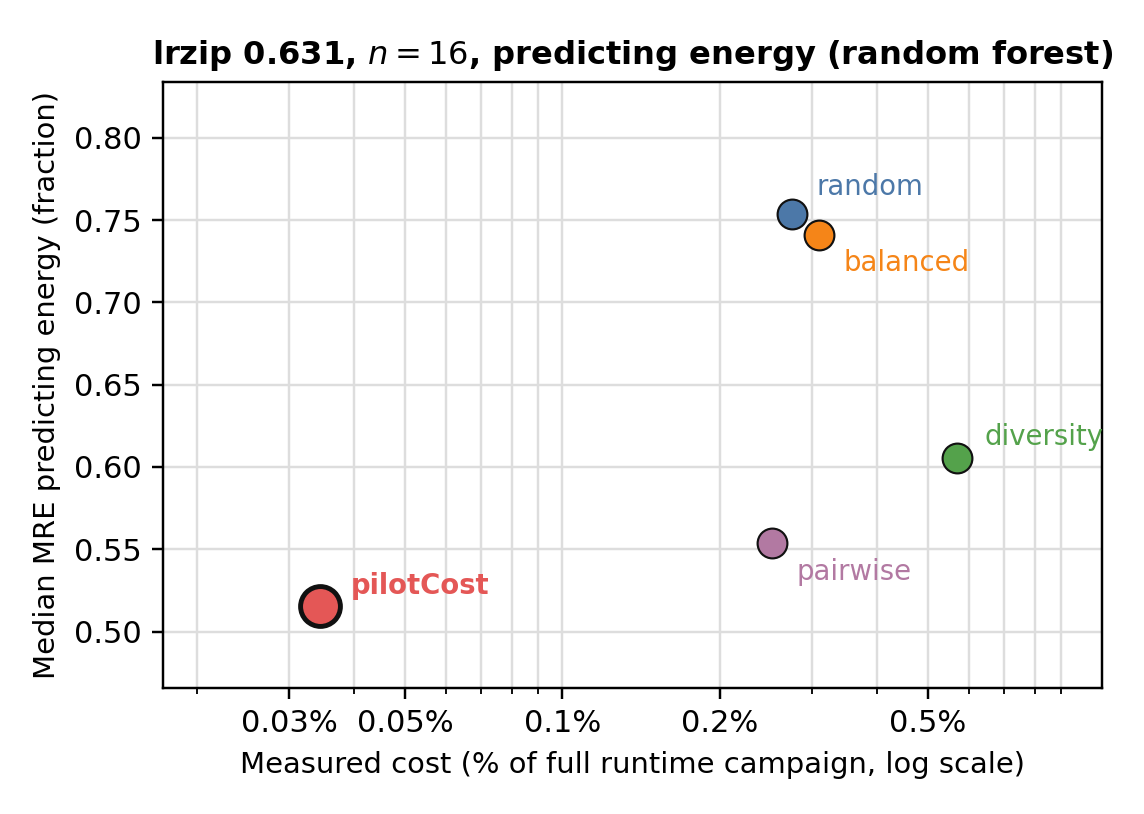
\includegraphics[width=0.75\linewidth]{pic/results/lrzip_fig1_rf_strictwin.png}
\caption{Same count, $>$order-of-magnitude measured-cost spread.}
\label{fig:re-scatter}
\end{subfigure}
\caption{Running example (lrzip 0.631, predicting energy under a measured-runtime
budget, random forest). (a) three of each strategy's $16$ measured
configurations: runtime (ms) is the per-point cost, energy (J) the label fit.
(b) sample count prices all five strategies alike, yet measured cost
separates them by more than an order of magnitude, and the cheapest
(\texttt{pilotCost}) is also the most accurate (learner-independent). Numbers in
text.}
\label{fig:running-example}
\end{figure*}

%The issue is not merely accounting. 
\Cref{fig:running-example} illustrates why treating sample size as a proxy for acquisition cost can be misleading. 
\Cref{fig:re-table} shows a subset of the sampled configurations ($n=3$ for \texttt{pilotCost} and \texttt{diversity}) on the lrzip subject from our performance-energy corpus.
%\Cref{fig:running-example} gives the smallest version of the phenomenon on a real subject: lrzip in the performance--energy corpus, where the goal is to predict energy but the budget is the measuredperformance cost of the training configurations (\Cref{fig:re-table}). 
\Cref{fig:re-scatter} summarizes the practical consequence ($n=3$ for five sampling strategies).
While all strategies measure the same $16$ configurations, so count-based effort assigns them
the same cost. Measured cost does not: \texttt{pilotCost}
spends only $0.03\%$ of the full budget while \texttt{diversity} spends $0.56\%$, a
$16.5\times$ gap counting cannot see, and \texttt{pilotCost} is also \emph{more
accurate} ($0.52$ vs.\ $0.61$ MRE, reported throughout as a fraction), strictly
dominating diversity on both axes. The reordering is not confined to the extremes:
\texttt{random} and \texttt{balanced} are cheaper than \texttt{diversity} yet less
accurate, a genuine cost--accuracy trade-off the count view hides. Sample size can
thus hide an order-of-magnitude cost difference, and even hide which strategy is
better, once cost is measured. Thus, our question is
not only whether $n$ correlates with cost in aggregate, but whether $n$ is a valid
cost axis for the sampling strategies a paper recommends, and whether the reversal
it shows is an isolated artifact of \Cref{fig:running-example} or a broader threat.

This paper's thesis is as follows: Sample size can order sampling effort, but treating it as the cost axis
is unsafe until the measured cost has been checked. In many
realistic scenarios, considering the actual cost changes the sampling strategy recommendation or the
set of efficient strategy--budget combinations.
This is not a blanket criticism of prior work. Sample size is practical,
reproducible, and often correlated with actual cost. Our claim is narrower:
when a paper makes a resource claim, the count proxy should be confronted against
the measured cost. A statement such as ``strategy $A$ is cheaper
than strategy $B$'' is only meaningful after specifying whether ``cheaper''
means fewer configurations or less measured cost.

We test the size-as-cost abstraction by replacing count-based effort with the
\emph{measured cost} of a strategy's training sample: the sum of the
per-configuration costs actually measured to acquire it, written $\TrainCost$.
This measured cost is the sampling cost our title sets against sample size. We
also call it an \emph{acquisition cost} when the point is what the resource is
spent on, namely the labels acquired for training, and otherwise use the shorter
\emph{measured cost} throughout. We study six families of experiments: (i) a
\StudyReplicationICSE revisit of Kaltenecker-style configurable-system
traces~\cite{kaltenecker2019}, (ii) a \StudyReplicationICPE revisit of x264~\cite{pereira2020}, %over $17$ inputs and two targets~\cite{pereira2020}, 
(iii) a performance--energy
corpus~\cite{weber2023twins}, (iv) a workload-impact corpus with $93$
system--workload contexts~\cite{muhlbauer2023workload}, (v) an \StudyLCBench
external-validation corpus with $35$ OpenML datasets and runtime learning
curves~\cite{zimmer2021autopytorch}, and (vi) six Linux kernel
releases~\cite{martin2022linux,borges2025linux}. We ask three research questions:
\emph{(1)}~to what extent sample size reflects measured cost,
\emph{(2)}~whether replacing sample size by measured cost changes
sampling-strategy conclusions, and \emph{(3)}~under which conditions sample size
is a safe or unsafe cost proxy. Agreement or disagreement across families is
itself part of the result.

The novelty is not the observation that configurations have heterogeneous
cost. %That much is expected. 
It is that the standard sample-count effort axis,
re-evaluated under measured cost, changes \emph{which samplers are
statistically recommendable} and \emph{which strategy--budget menus are
Pareto-efficient}, established with the original studies' own statistical test
rather than a new one of our choosing. Our contributions are as follows:

% \noindent\textbf{Contributions.}
\begin{itemize}
    \item We operationalize measured cost as an evaluation axis and
    define metrics that test
    when sample size can stand in for it.
    \item We quantify the decision impact by re-running the replication studies'
    own Kruskal--Wallis sampler test and Pareto choice-set analysis under measured
    cost, which change both the statistically recommendable samplers and the
    efficient strategy--budget menu.
    \item We show that measuring cost surfaces \emph{cost-aware} samplers that
    are off the radar under sample count, and give an existence proof:
    \texttt{pilotCost}, a deliberately simple pilot of cost-aware sampling, is on
    several systems the most cost-effective choice: better accuracy at equal sample size.
    %measured cost.
    \item We identify validity conditions and reporting guidance: count-based
    conclusions are most defensible on homogeneous, cost-unaware regimes, and
    fragile under heavy-tailed costs, target--cost asymmetry, workload/context
    shifts, and diversity or active-learning samplers.
\end{itemize}
